%!TEX root = ../erweiterte_sachkunde.tex
\chapter{Anatomie und Physiologie des Hundes}


\section{Allgemeiner Aufbau und anatomische Lage}

    \subsection{Bewegungsapparat mit Knochen, Muskeln und Gelenken}
    \begin{figure}[ht]
    \centering
    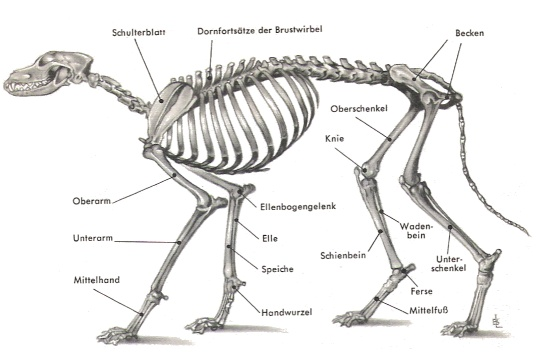
\includegraphics[width=1.0\textwidth]{./bilder/anatomie1.jpg}
    \caption{Skelett}
    \label{Skelett}
    \end{figure}

    \clearpage
    Ergänzend zu Abbildung \ref{Skelett} Skelett:
    \begin{itemize}
        \item Wirbelsäule: Halswirbelsäule, Lendenwirbelsäule, Kreuzbein, Rute
        \item Brustkorb mit 13 Rippenpaaren
        \item Hintergliedmaßen: befestigt am Becken, bestehend aus:
        \begin{itemize}
            \item Darmbein
            \item Schambein
            \item Sitzbein
        \end{itemize}
    \end{itemize}

    \begin{figure}[ht]
    \centering
    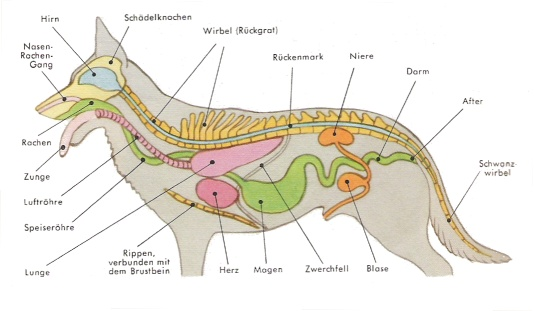
\includegraphics[width=1.0\textwidth]{./bilder/anatomie2.jpg}
    \caption{Organe}
    \label{Organe}
    \end{figure}

    Ergänzend zu Abbildung \ref{Organe} Organe:
    \begin{itemize}
        \item Brustkorb (Thorax):
        \begin{itemize}
            \item Brusthöhle nach hinten von Zwerchfell begrenzt, welches im Brustkorb liegt. Deshalb ist der Brustkorb größer.
            \item Brusthöhle beinhaltet Herz und Lunge. Dort herrscht Unterdruck, damit sich die Lunge entfalten kann.
            \item Zusätzlich: Leber und Magen (Zählen zu Bauchorgane)
        \end{itemize}
        \item Bauch (Abdomen):
        \begin{itemize}
            \item Magen-Darm-Trakt
            \item Bauchanhangdrüsen: Leber und Bauspeicheldrüse
            \item Milz
        \end{itemize}
        \item Beckenhöhle: begrenzt von Kreuzbein und Becken.
        \begin{itemize}
            \item Harnorgane
            \item Geschlechtsorgane
        \end{itemize}
    \end{itemize}


\section{Einzelheiten}

    \subsection{Haut und Fell}
    \begin{itemize}
        \item Schutz vor Austrocknung, Parasiten, Bakterien und Viren
        \item Temperaturregulation beim Hund über Hecheln. Es sind keine Schweißdrüsen unter der Haut wie beim Menschen vorhanden.
        \item Normaltemperatur: 38-39 Grad
    \end{itemize}

    \subsection{Kopf}
    \begin{itemize}
        \item Augen: Sehschärfe wie beim Menschen, Rot-Grün-Farbblindheit
        \item Ohren: Inneres Ohr mit Flüssigkeit gefüllt, Gleichgewichtsorgan
        \item Nase: sehr empfindlich, sehr gut ausgebildet
        \item Mund: Schutz beim Erbrechen vor Magensäure, da alkalische Eigenschaften \\
              Zähne:
        \begin{itemize}
            \item 42 (22 im Oberkiefer, 20 im Unterkiefer)
            \item Welpen: 28, Milchzähne ab 2.-3. Woche
            \item Zahnwechsel: 2 - 6 Monate
        \end{itemize}
        \item Kreuzung von Speise- und Atemwege. Beim Schlucken werden Nasenraum und Kehlkopf verschlossen, damit kein Futterbrei in die Atemwege gelangt
    \end{itemize}

    \subsection{Hals}
    \begin{itemize}
        \item Luftröhre: Reinigt, befeuchtet und erwärmt die Atemluft
        \item Speiseröhre: stark dehnbar
    \end{itemize}

    \subsection{Brusthöhle}
    \begin{itemize}
        \item Herz: 2 Vorhöfe, 2 Kammern
        \item Lunge
    \end{itemize}

    \subsection{Bauchorgane}
    \begin{itemize}
        \item Leber: liegt direkt hinter dem Zwerchfell, Stoffwechsel, Speichern von Blutzucker, Entgiftung
        \item Magen:
        \begin{itemize}
            \item sehr dehnbar
            \item Muskelteil zur Zerkleinerung von Futter
            \item Drüsenteil mit Enzymen für die Verdauung
            \item Aufhängeapparat relativ locker, deshalb Neigung zur Magendrehung
        \end{itemize}
        \item Darm:
        \begin{itemize}
            \item Übergang Magen $\rightarrow$ Dünndarm auf der rechten Seite
            \item Mündung der Bauchspeicheldrüse (gibt Enzyme für die Verdauung ab)
            \item Dünndarm: weitere Verdauung und Aufnahme von Einzelstoffen ins Blut
            \item Dickdarm:
            \begin{itemize}
                \item Aufnahme von Wasser des Darms ins Blut
                \item Eindickung des Kotes
                \item Ausscheidung
            \end{itemize}
            \item Milz:
            \begin{itemize}
                \item linke Bauchwand
                \item Abbau von roten Blutkörperchen und -plättchen
                \item Immunabwehr
                \item Blutbildung bei Jungtieren
            \end{itemize}
        \end{itemize}
    \end{itemize}

    \subsection{Organe der Beckenhöhle}
    \begin{itemize}
        \item Harnapparat:
        \begin{itemize}
            \item Nieren:
            \begin{itemize}
                \item Reinigung des Blutes
                \item Umwandlung zu Harnstoff
                \item Regulation des Wasserhaushalts + Blutdrucks
            \end{itemize}
            \item Harnleiter
            \item Harnblase
            \item Harnröhre:
            \begin{itemize}
                \item Mündung weiblicher Geschlechtsorgane
                \item Rüden: getrennte Ausführungsgänge im Penis für Samen und Urin
            \end{itemize}
        \end{itemize}
        \item Geschlechtsapparat:
        \begin{itemize}
            \item Weiblich:
            \begin{itemize}
                \item Paarige Eierstöcke an der Spitze der Gebärmutter
                \item Gebärmutterhals geht in Vagina über. Reifung der Frucht, Hormonproduktion
                \item Östrogen: Läufigkeit (4 - 12 Tage)
                \item Progesteron: Trächtigkeit (63 Tage)
                \item Besamungzeitpunkt: 2-3 Tage nach Ende der Läufigkeit
                \item Scheinträchtigkeit:
                \begin{itemize}
                    \item Nicht erfolgte Belegung führt trotzdem zu Mutterinstinkten ca. 2 Monate nach der Läufgkeit (wie bei einer gedeckten Hündin).
                    \item Keine Krankheit, sondern hormonell bedingt
                    \item Trotzdem Gefahr von Milchstau.
                    \item Milderung: Ablenken, Spaziergänge etc.
                \end{itemize}
            \end{itemize}
            \item Männlich: Penisknochen (Typisch beim Hund)
        \end{itemize}
    \end{itemize}


\section{Ausgewählte Erkrankungen}

    \subsection{Entzündung allgemein}
    \begin{itemize}
        \item Kann in jedem Körperteil bei Viren-/Bakterien- oder Parasietenbefall auftreten
        \item Symptome: Rötung, Schwellung, Schmerz, vermehrte Wärme
    \end{itemize}

    \subsection{Durchfall}
    \begin{itemize}
        \item Komplex
        \item Mögliche Ursachen: Stress, Futterumstellung, Bakterien, Viren, Parasiten
        \item Kann auch von \glqq Leckerchen\grqq{} ausgelöst werden
    \end{itemize}

    \subsection{Magendrehung}
    \label{ch:Anatomie:sec:Erkrankungen:subsec:Magendrehung}
    \begin{itemize}
        \item Notfall! Führt ohne sofortige OP zum Tod
        \item Betroffen sind vor allem große Rassen
        \item Auslösende Faktoren: Herumspringen nach Nahrungsaufnahme, Verfütterung von verdorbenem oder gährungsfähigem Futter
        \item Starke Blähung des Magens und danach Drehung um 180 Grad
        \item Typische Anzeichen:
        \begin{itemize}
            \item meist abends
            \item Hund ist unruhig und teilnahmslos zugleich
            \item Hecheln, Speicheln, Versuch zu Erbrechen
            \item aufgeblähter Bauch
            \item Schock
        \end{itemize}
        \item Nach der OP: 3 kritische Tage
        \item Vorbeugen: mehrmals täglich kleinere Portionen oder Ruhe nach dem Fressen
    \end{itemize}

    \subsection{Pyometra}
    \begin{itemize}
        \item Gebärmuttervereiterung, kann zum Tode führen
        \item Zeitpunkt: 4-8 Wochen nach der letzten Läufigkeit
        \item Symptome:
        \begin{itemize}
            \item Schwäche der Hinterhand
            \item Apathie
            \item Futterverweigerung
            \item Durst und Harndrang nehmen zu
            \item Zwei Arten:
            \begin{itemize}
                \item offen: Eiterausfluss aus der Scheide
                \item geschlossen: angespannte Bauchdecke
            \end{itemize}
        \end{itemize}
        \item Therapie: Kastration
    \end{itemize}

    \subsection{Zahnstein}
    \begin{itemize}
        \item Symptome: Verfärbung und Auflagerung der Zähne
        \item Verursacht möglichwerwiese Zahnschmerzen, Fressprobleme, Herzerkrankungen
    \end{itemize}


\section{Impfungen}

    \subsection{Impfprogramm}
    \begin{tabular}{c|l}
        \textbf{Zeitpunkt} &   \textbf{Impfung} \\
        \hline
        6 Wochen    & Parvovirose (bei erhöhtem Infektionsdruck) \\
        8 Wochen    & Staupe, Hepatitis, Parvo, Leptospirose \\
                    & bei erhöhtem Infektionsdruck auch Zwingenhusten \\
        12 Wochen   & Wiederholungsimpfung \\
        16 Wochen   & Tollwutimpfung \\
        Jährlich    & Wiederholungsimpfungen \\
    \end{tabular}

    \subsection{Parvovirose}
    \begin{itemize}
        \item Viruserkrankung (v.a. Bullterrier, Dobermann, Labrador, Rottweiler)
        \item Inkubationszeit: 4-14 Tage
        \item Symptome Erbrechen, Fieber, Durchfall, Austrocknen \\
              Jungtiere: Herzkrankheiten, Blutvergiftung, Bauchspeicheldrüsenentzündung
        \item Übertragung: Kot, sehr resistent (bis 6 Monate), symptomlose Wirtshunde möglich
    \end{itemize}

    \subsection{Staupe}
    \begin{itemize}
        \item Viruserkrankung: Atmungstrakt, Magen-Darm-Trakt, Nervensystem
        \item Inkubationszeit 8 Wochen - 6 Monate
        \item Symptome: Erbrechen, Fressunlust, Durchfall, eitriger Nasenausfluss, Husten, Lähmungen, später Verhornung der Nase und Zehenballen
        \item Übertragung: Ausscheidungen
    \end{itemize}

    \subsection{Hepatitis}
    \begin{itemize}
        \item Viruserkrankung
        \item Inkubationszeit: 4 - 8 Tage, manchmal inerhalb von Stunden
        \item Symptome: Fieber, Apathie, Erbrechen
        \item Übertragung: Kot
    \end{itemize}

    \subsection{Leptospirose}
    \begin{itemize}
        \item Bakterielle Erkrankung,
        \item auf Menschen übertragbar (Zoonose), meldepflichtig
        \item Symptome: Fieber, Steifheit, Erbrechen, Durchfall, vermehrtes Trinken und urinieren, erschwertes Atmen, kleine Blutungen auf den Schleimhäuten
        \item Übertragung: Über Urin von Nagern, gegenseitiges Belecken, Bisswunden, stehendes/lauwarmes Wasser
    \end{itemize}

    \subsection{Tollwut}
    \begin{itemize}
        \item Viruserkrankung
        \item meldepflichtige Zoonose
        \item Übertragung: Bisse infizierter Tiere
        \item Inkubationszeit: wenige Wochen - 8 Monate
        \item Impfpflicht für das Mitnehmen des Hundes ins Ausland
        \item Impfschutz erst 21 Tage nach Impfung
    \end{itemize}